\chapter{Application web}

	\section{Organisation des packages}

		\subsection{Packages}

			%TODO Léa : Image et décrire le but des packages (src)

			L'organisation des packages se présente comme suit :

			\begin{figure}[H]
				\centering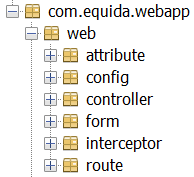
\includegraphics[width=0.33\textwidth, keepaspectratio]{res/webapp-package.png}
				\caption{Packages de WebApp}
			\end{figure}

			\begin{description}
				\item[attribute :]{Contient la classe InputOutputAttribute qui gère toutes les constantes dont on pourrait avoir besoin}
				\item[config :]{Contient les classes relatives à la configuration et la sécurité de l'application}
				\item[controller :]{Contient toutes les contrôleurs qui héritent de la classe AbstractWebController}
				\item[form :]{Contient tous les formulaires qui héritent de la classe IForm}
				\item[interceptor :]{Contient la classe UserInterceptor qui hérite de HandlerInterceptorAdapter (voir \nameref{subsec:interceptor} et/ou \url{https://www.tutorialspoint.com/spring_boot/spring_boot_interceptor.htm})}
				\item[route :]{Contient toutes les routes qui héritent de IRoute}
			\end{description}

		\subsection{Resources}

			%TODO Léa : Comme avec les packages mais sur les ressources

			L'organisation des ressources se présente comme suit :

			\begin{figure}[H]
				\centering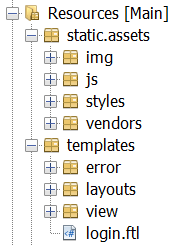
\includegraphics[width=0.33\textwidth, keepaspectratio]{res/ressources.png}
				\caption{Ressources de WebApp}
			\end{figure}

			\begin{description}
				\item[static.assets :]{Contient toutes les ressources statiques qui ne nécessitent aucune compilation}
				\begin{description}
					\item[img :]{Contient toutes les images de l'application}
					\item[js :]{Contient tous les fichiers JavaScript notamment celui pour la gestion des classements à une course d'un cheval et celui pour la page d'accueil avec son carrousel et son menu}
					\item[styles :]{Contient le fichier css de base}
					\item[vendors :]{Contient toutes les dépendances externes du projet soit : Materialize (librairie qui gère le design des vues de l'application), jQuery, Google (police de caractères)}
				\end{description}

				\item[templates :]{Contient tous les fichiers Freemarker}
				\begin{description}
					\item[error :]{Contient les fichiers ftl pour les erreurs 403, 404, 500}
					\item[layouts :]{Contient les fichiers ftl communs à toutes les pages de l'application}
					\item[view :]{Contient toutes les vues de l'applications (lister, consulter, form)}
					\item[login.ftl :]{Fichier utilisé par SpringSecurity pour la page d'authentification}
				\end{description}
			\end{description}

	\section{Parler configuration de l'application}

		\subsection{application.properties}

			%TODO Justine

		\subsection{Configuration par le code}

			%TODO Justine

	\section{Fichiers resources}

		\subsection{FreeMarker}
			FreeMarker est un moteur de template basé sur Java qui est à l'origine de la génération de pages web dynamiques dans une architecture logicielle.\newline
			FreeMarker lit donc les fichiers Model, les combine avec les objets Java pour finalement générer un document de sortie type HTML (dans un format de fichier FTL FreeMarker Template Language).

			\subsubsection{Page de base}

				%TODO Léa : Expliquer le fonctionnement de la page de base et les macros
				La page base.ftl correspond à la page type de l'application. On y retrouve ainsi ce qui sera inclus sur toutes les pages de l'application. \newline
				Ainsi, base.ftl contient le header de la page avec l'inclusion de la feuille de style ; sa partie body contient, elle, le contenu du fichier nav.ftl correspondant au menu, ainsi que le footer et les fichiers de scripts nécessaires.\newline
				Les macros permettent le chargement du contenu aux endroits prévus à cet effet. Par exemple, la drective <@content/>, présente dans le body de base.ftl, chargera le code dans la macro "content" du fichier x.ftl à cet endroit.

				\begin{figure}[H]
					\centering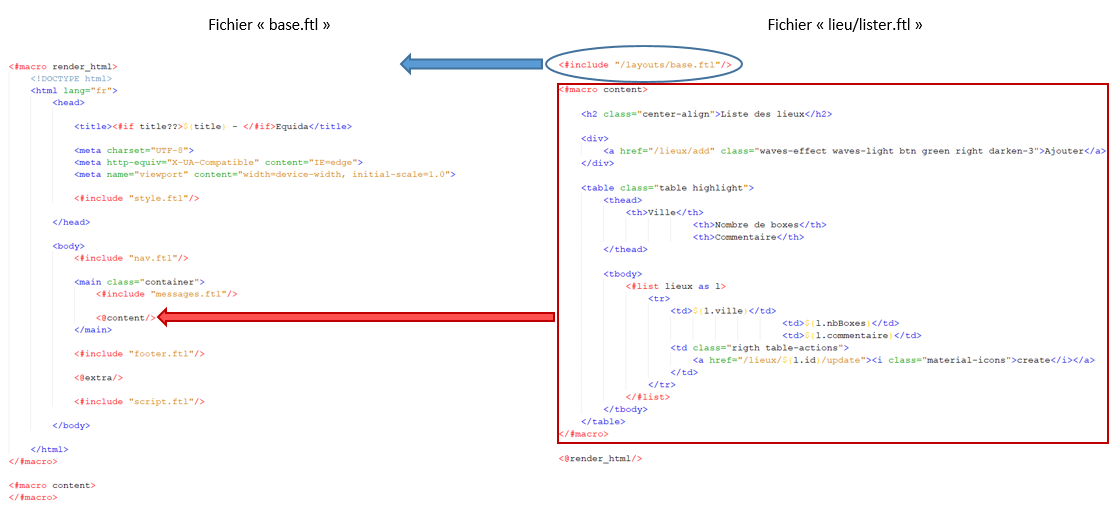
\includegraphics[width=1\textwidth, keepaspectratio]{res/fonctionnementBaseFtl.png}
					\caption{Exemple du fonctionnement de la page base.ftl avec la page lieux/lister.ftl}
				\end{figure}

				\begin{figure}[H]
					\centering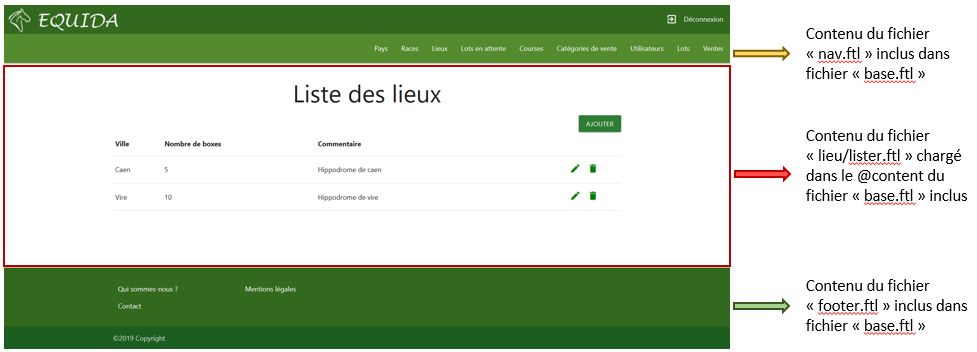
\includegraphics[width=1\textwidth, keepaspectratio]{res/exempleFonctionnementBaseLieuFtl.png}
					\caption{Rendu lors du chargement de la vue qui liste les lieux (correspondant à la page lieux/lister.ftl précédente)}
				\end{figure}

			\subsubsection{Page d'erreur}

				%TODO Léa : Expliquer que les pages sont chargés automatiquement par spring et reprenne design de base
				Les pages d'erreur sont chargées automatiquement par Spring et contiennent des messages explicites. Nous avons gérés les erreurs 403 (permissions non autorisées), 404 (page inexistante) et 500 (exception lors de l'exécution du code). Elles reprennent, elles aussi, le design de base de l'application (base.ftl).

				\begin{figure}[H]
					\centering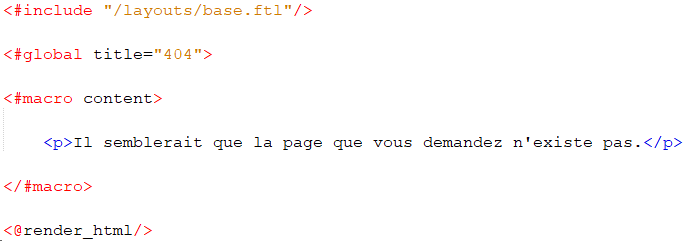
\includegraphics[width=0.75\textwidth, keepaspectratio]{res/codeErreur404.png}
					\caption{Code de l'erreur 404}
				\end{figure}

				\begin{figure}[H]
					\centering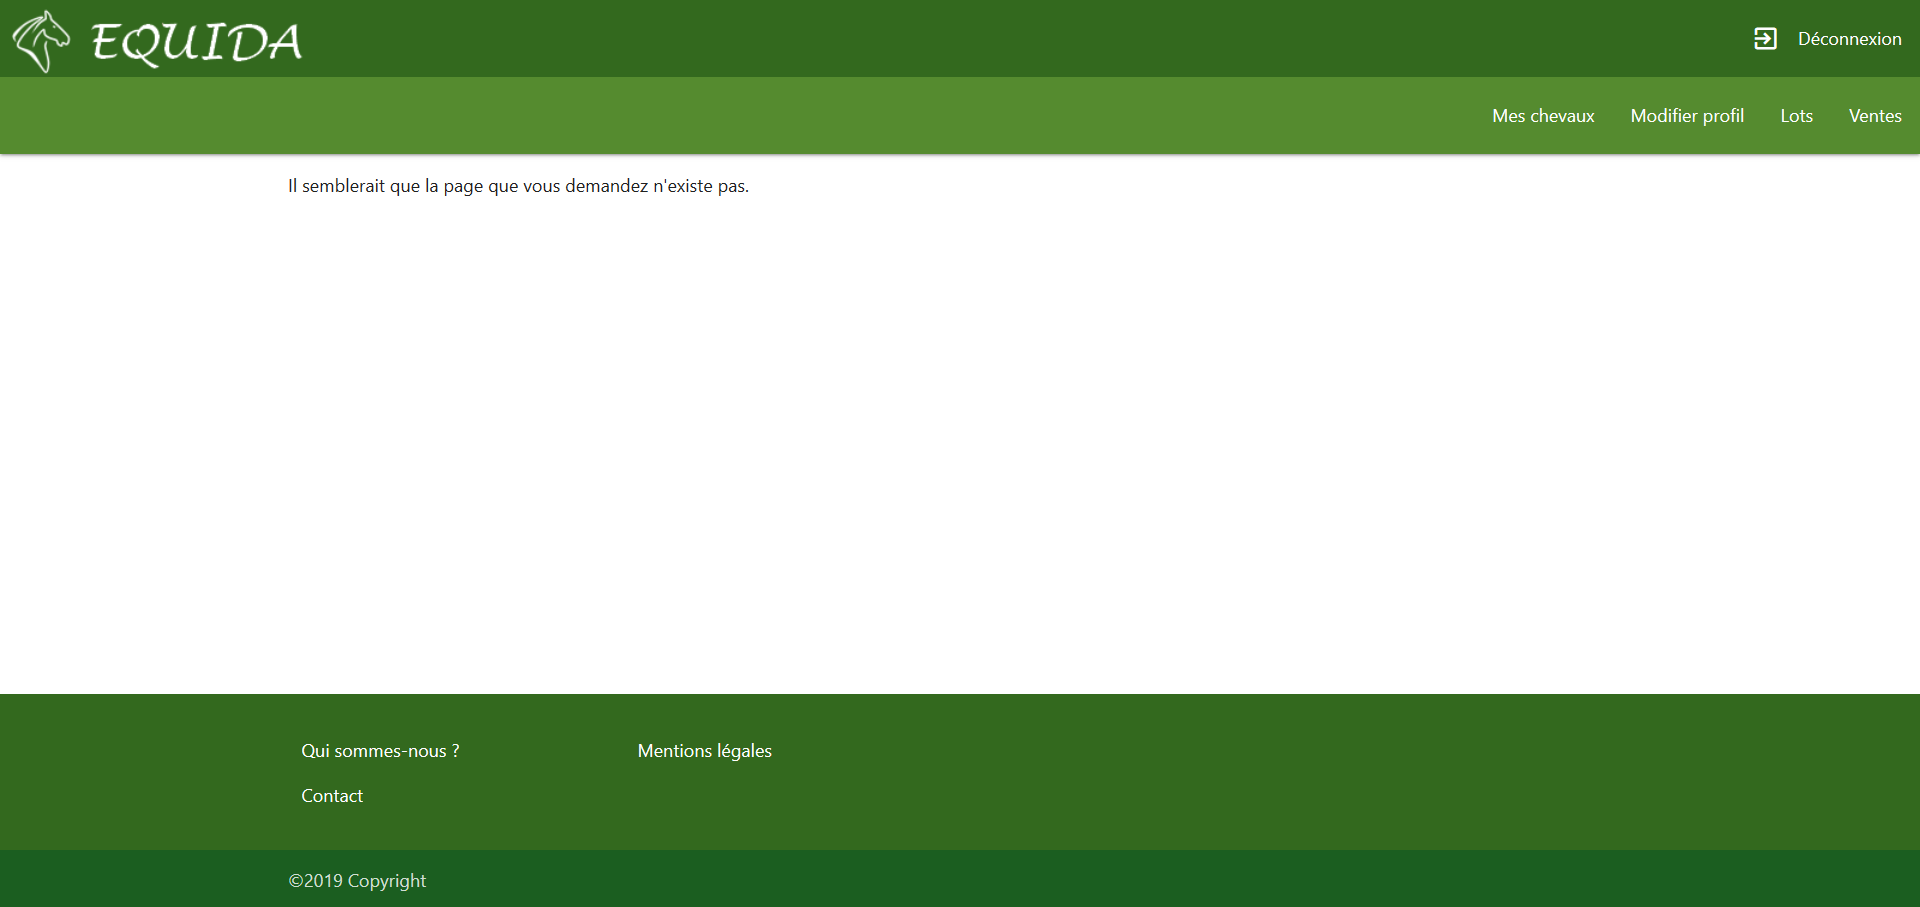
\includegraphics[width=0.85\textwidth, keepaspectratio]{res/exempleErreur404.png}
					\caption{Rendu lors d'une tentative de chargement d'une page inexistante}
				\end{figure}

			\subsubsection{Autre}

				%TODO Justine : Fichiers include + fichiers normaux

	\section{Parler authentification}

		\subsection{Gestion template et controller}

			%TODO Justine

		\subsection{Interceptor}
			\label{subsec:interceptor}

			%TODO Justine

	\section{Exemple Route}

		%TODO Léa : Expliquer les méthodes de l'interface IRoute et donner un exemple de route.
		L'interface IRoute décrit les méthodes qui doivent être implémentées par les classes filles.\newline
		Ainsi chaque fichier route contiendra une méthode getUri(), une méthode getView() et getTitle() qui retourneront respectivement l'URL, la vue et le titre à utiliser dans la page concernée (pour la route correspondante).

		\noindent
		Par exemple, pour PaysRoute, qui est donc la route principale selon notre nomenclature, l'URL correspond à /pays, c'est à cette url là, qu'on chargera la vue pays/lister avec le titre "Les pays".

		\begin{figure}[H]
			\centering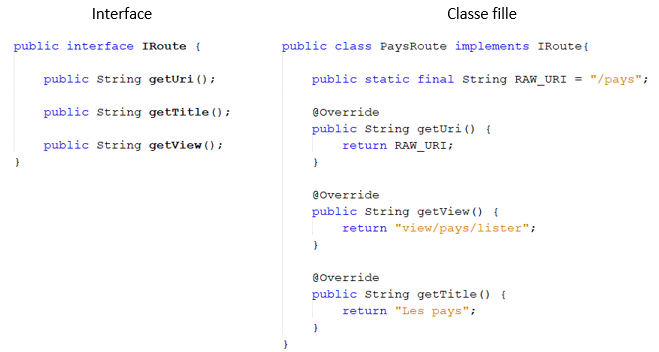
\includegraphics[width=0.75\textwidth, keepaspectratio]{res/paysRoute.png}
			\caption{Code de l'interface et utilisation par la classe fille PaysRoute}
		\end{figure}

		\begin{figure}[H]
			\centering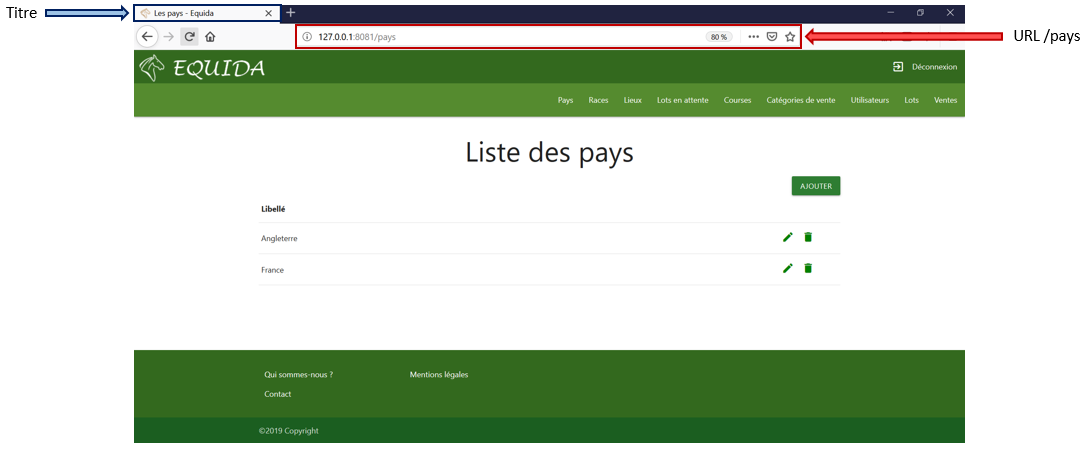
\includegraphics[width=0.85\textwidth, keepaspectratio]{res/renduPaysRoute.png}
			\caption{Rendu obtenu avec la vue pays/lister}
		\end{figure}

	\section{Exemple Form}

		%TODO Léa : Expliquer la classe mère IForm et donner un exemple de formulaire (Avec Add et Update et le Neutre)
		La classe mère IForm est une classe abstraite qui utilise la générécité ce qui nous permettra d'adapter les méthodes en fonction de l'entité x pour laquelle le formulaire est fait. L'héritage nous permet donc d'utiliser les variables et méthodes déclarées dans le formulaire neutre xForm.\newline
		Par exemple, prenons l'entité Lieu. On créé le formulaire "neutre" LieuxForm qui héritera de IForm et qui permettra de définir les éléments communs aux formulaire d'ajout et de modification.\newline
		On fera donc hériter de ce formulaire "neutre" LieuxAddForm et LieuxUpdateForm et on passera, dans un premier cas, le la variable isCreation à true et dans le second, à false.

		\begin{figure}[H]
			\centering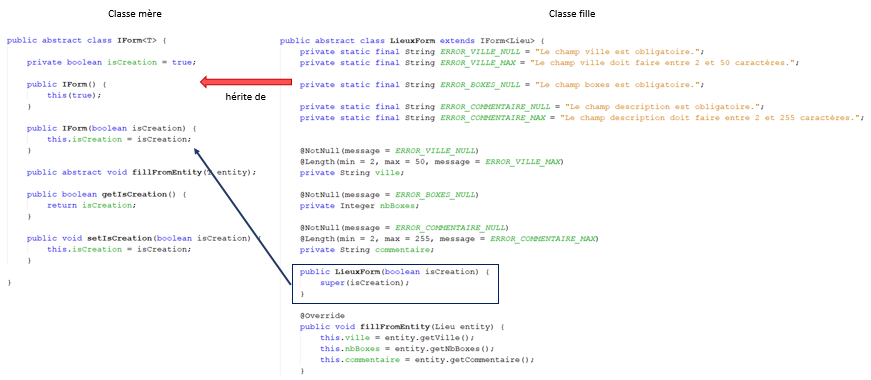
\includegraphics[width=1\textwidth, keepaspectratio]{res/IForm.png}
			\caption{Exemple implémentation interface IForm avec LieuxForm}
		\end{figure}

		\begin{figure}[H]
			\centering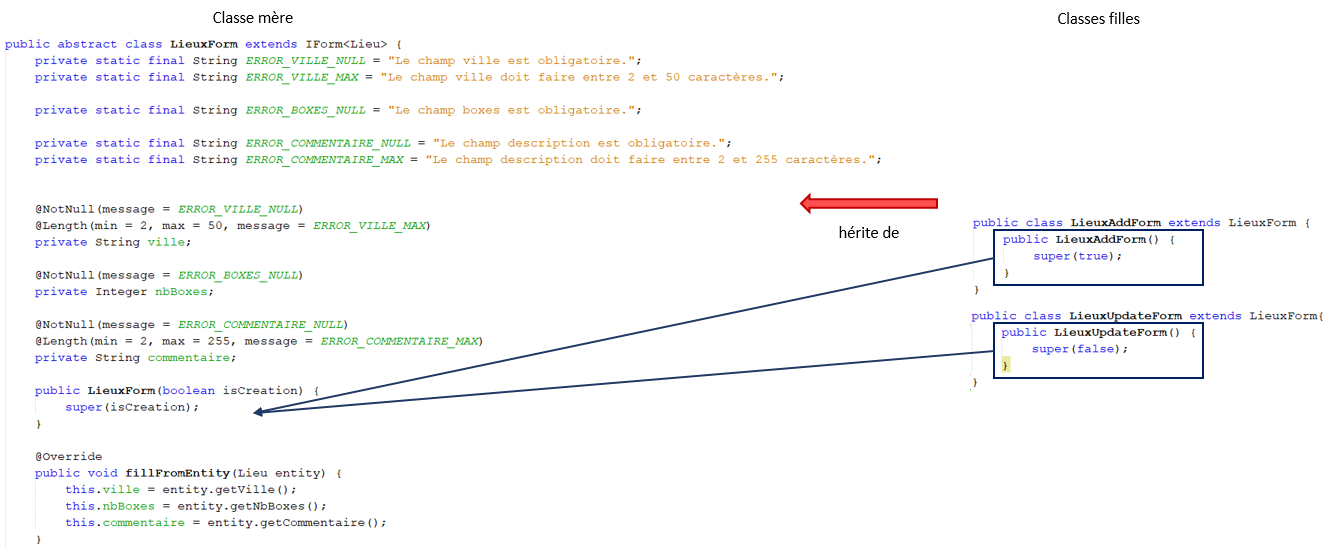
\includegraphics[width=1\textwidth, keepaspectratio]{res/formClassFilles.png}
			\caption{Exemple avec LieuxUpdateForm et LieuxAddForm}
		\end{figure}

	\section{Classe InputOutputAttribute}

		%TODO Justine

	\section{Exemple Controller}

		%TODO Léa : Donner un exemple de controller

		Les différents contrôleurs créés pour les entités x héritent tous de la classe AbstractWebController. \newline
		Les contrôleurs contiennent différentes méthodes associées aux méthodes GET, POST, PATCH et DELETE ainsi qu'a une route. Enfin elles utilisent les services pour intéragir avec la \bdd{}. On y définit aussi les différentes autorisations avec l'annotation @PreAuthorize afin de savoir qui peut accéder à la page, et donc, executer la méthode.

		\noindent
		Par exemple, dans EncheresController, la méthode addGet n'est possible que pour un utilisateur ayant le role 'ADMIN', elle est reliée à l'URL EncheresAddRoute.RAW\_URI (URL stockée dans la variable constante RAW\_URI de la classe EncheresAddRoute). Elle permet de récupérer les différentes variables nécessaires à l'affichage de la page, comme le formulaire d'ajout d'une enchère par exemple.

		\begin{figure}[H]
			\centering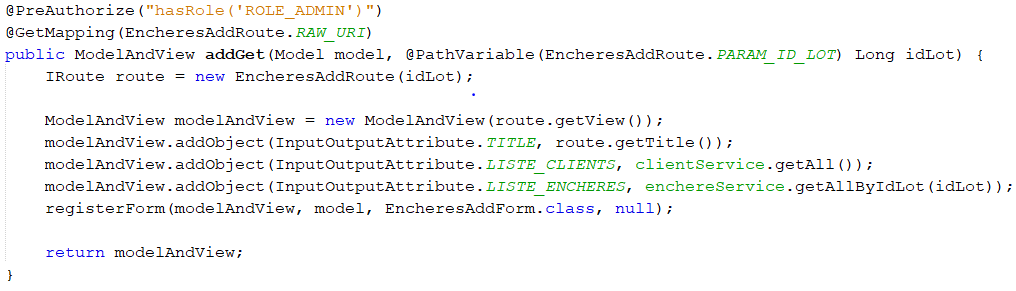
\includegraphics[width=0.75\textwidth, keepaspectratio]{res/enchereController.png}
			\caption{Exemple d'un contrôleur}
		\end{figure}
